% ---
% Arquivo com as especificações do Trabalho de Conclusão de Curso do aluno
% Daniel Noriaki Kurosawa
% da Escola Politécnica da Universidade de São Paulo
% ---
	% ---
		\chapter{Especificações}\label{cap-especificacao}
		
		
	Esta seção baseia-se nos 5 pontos fundamentais da ODP (Open Distributed Processing)	para especificar o projeto a ser desenvolvido. Assim, divide-se este capítulo em:	Visão Empresarial, de Informação, Computacional, de Engenharia/Infraestrutura e de Tecnologia.\par
		\section{Visão Empresarial}\label{sec-empresarial}
	\subsection{Monetização do projeto}\label{subsec-monetizacao}
		O projeto desenvolvido tem o intuito de possibilitar a interação imersiva com um ambiente remoto através do uso de câmeras estereoscópicas e da operação de um braço robótico. Analisando o projeto, encontramos usos distintos para suas partes componentes em separado, assim como usos envolvendo as duas partes.
		
		\subsubsection{Sistema de câmeras estereoscópico}	\label{subsubsec-cameras}
			\begin{itemize}
	\item Câmeras de Vigilância de Ambientes: é possível aplica-los ao utilizar mais de um conjunto de câmeras, uma vez que o usuário tem a possibilidade de assinalar um endereço independente para cada um deles.
	
	\item Câmeras de Entretenimento: ao possibilitar o acompanhamento visual baseado na movimentação da cabeça do usuário, é possível dar acesso a áreas restritas de locais como exposições, zoológicos, aquários e áreas sensíveis a concentração de pessoas através das câmeras instaladas, permitindo uma experiência exclusiva em tais locais. 
	\end{itemize}
		\subsubsection{Braço mecânico}\label{subsubsec-braco}
	\begin{itemize}
	\item Programação de braços robóticos industriais : Caso seja desenvolvido um software para o armazenamento dos dados de movimentação do usuário, é possível a utilização do projeto para uma rápida automatização de uma tarefa repetitiva.
	\end{itemize}	
	\subsubsection{Projeto como um todo}\label{subsubsec-all}
	\begin{itemize}
	\item Desarmamento de Explosivos: pode ser utilizado em operações de reconhecimento em locais remotos e no desarmamento de explosivos, proporcionando uma maior segurança aos operadores.

    \item Operações Médicas à Distância:  Este tipo de abordagem pode oferecer novas alternativas para operações à distância mais eficazes e flexíveis, dando a locais com escassez de recursos acesso a serviços médicos. Para tal aplicação no entanto, são necessárias melhorias na precisão do hardware/software.
    
	\item Jogos de Realidade Aumentada: o projeto pode ser viabilizado neste campo, dando uma experiência imersiva ainda mais enriquecedor ao usuário não só no ambiente virtual, mas também no ambiente real mostrando um grande potencial na criação de novas dinâmicas de jogos e entretenimento.
	\end{itemize}
	
	

	


	
	\section{Visão de Informação}\label{sec-info}
	\subsection{Elementos de informação do sistema}\label{subsec-elementos-info}
	
		\begin{figure}[h!]
		\caption{\label{fig_eleminfo}  Elementos de informação do sistema}
		\begin{center}
			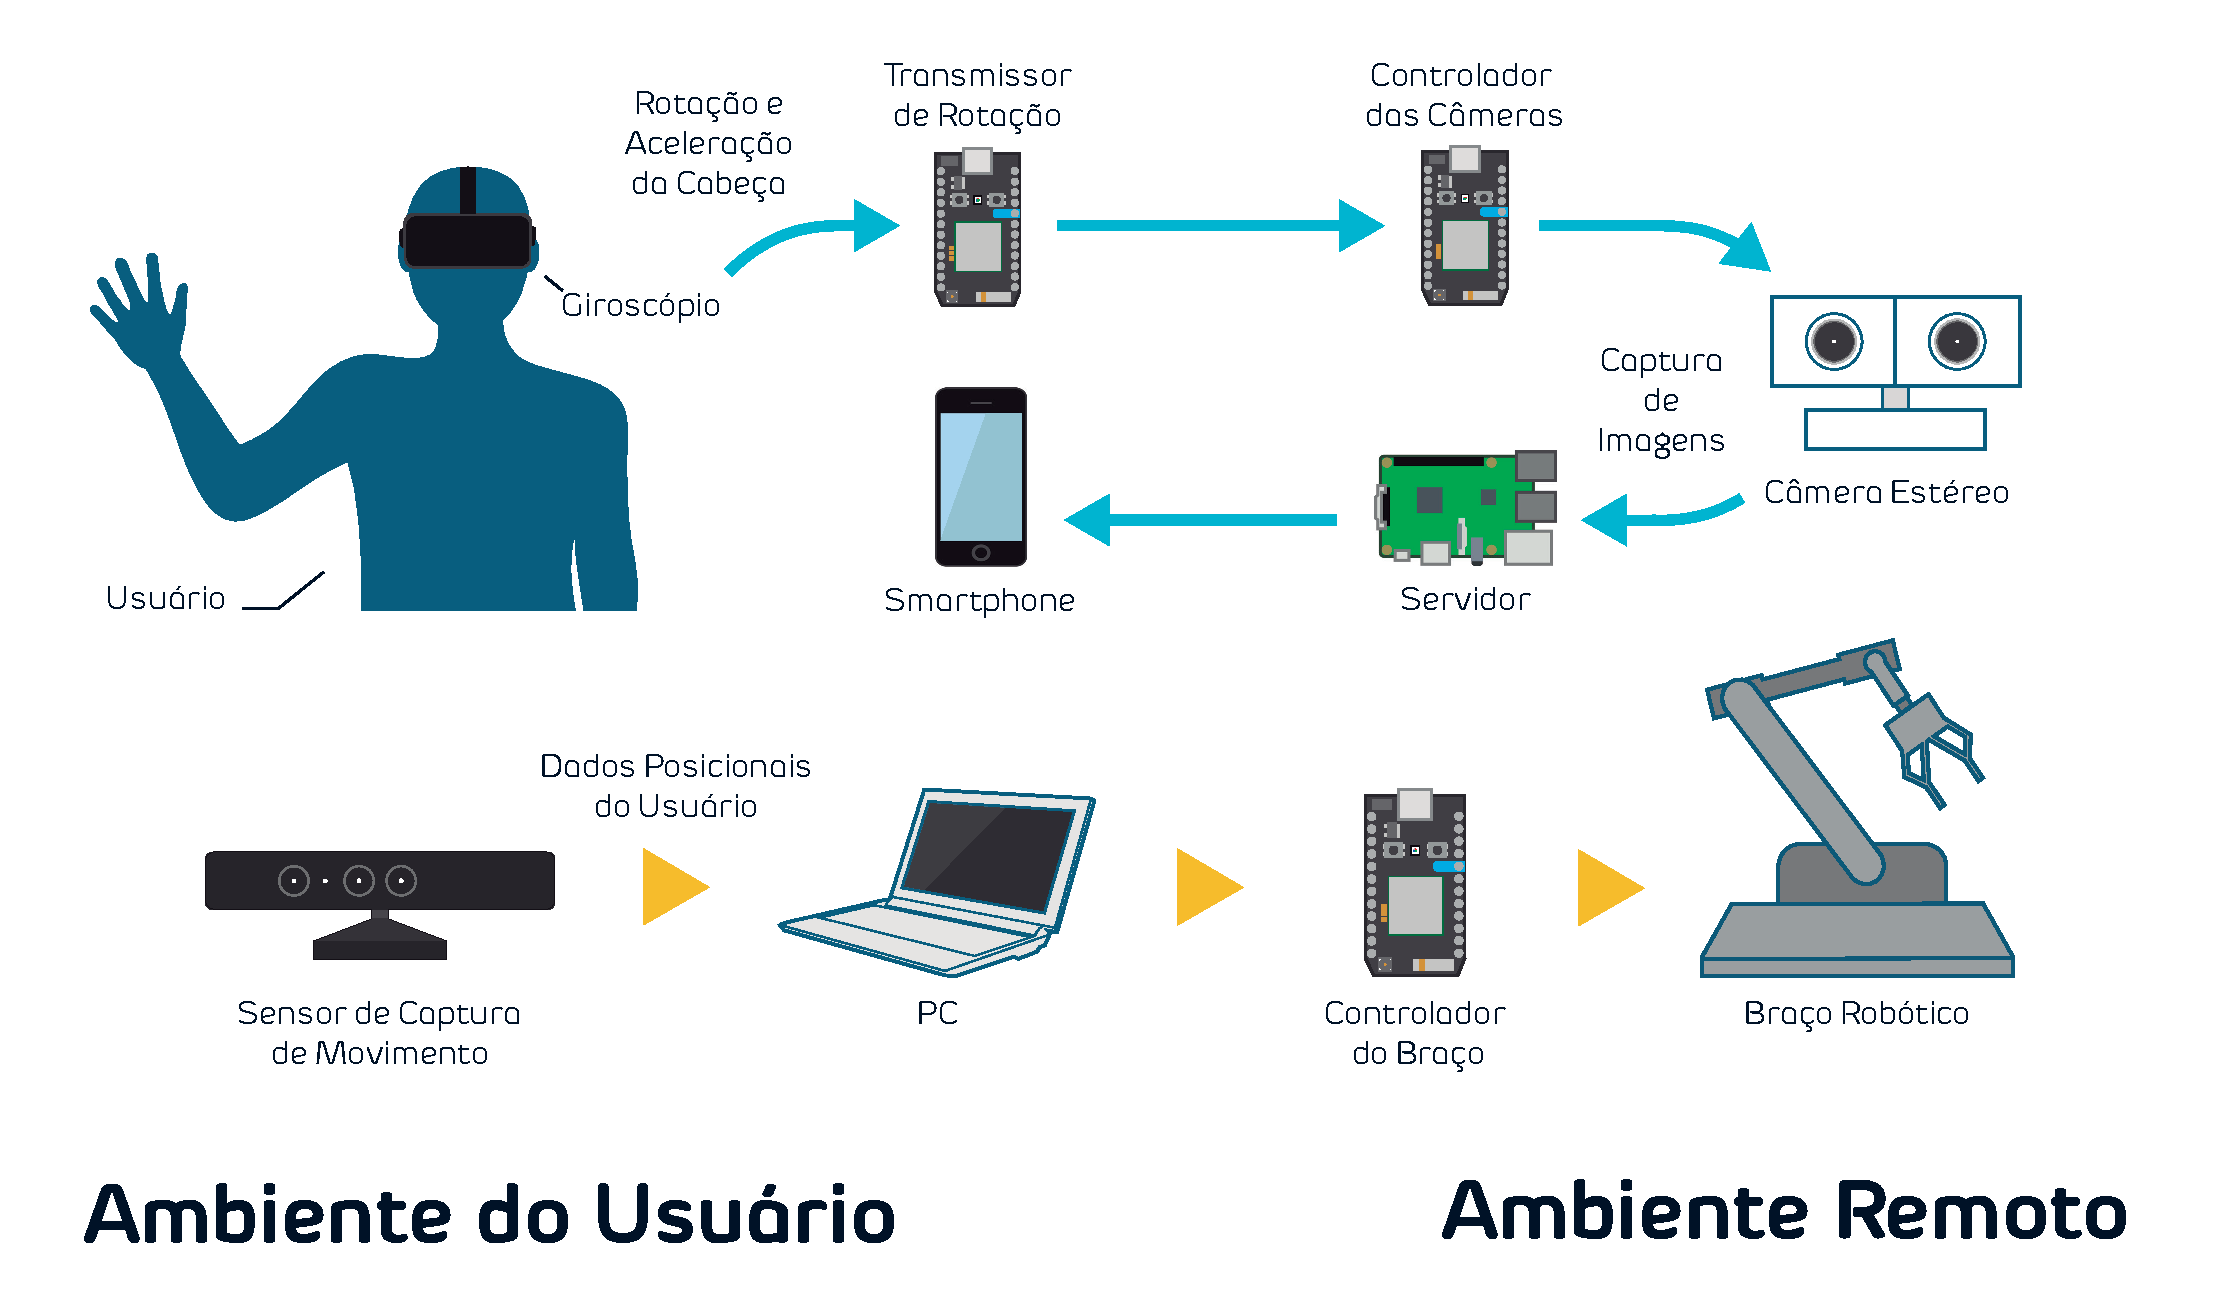
\includegraphics[width=\textwidth]{eleminfo.pdf}	
		\end{center}
		\legend{Fonte: Autor}
	\end{figure}
	
	Para facilidade de compreensão, esta subseção se divide em três partes:
	\subsubsection{Rotação e aceleração da cabeça do usúario}\label{subsubsec-elementos-info-rotation}
	Os movimentos verticais e horizontais da cabeça do usuário são coletados e convertidos em valores numéricos de aceleração e ângulo através do giroscópio GY-521 acoplado na parte traseira do óculos de realidade virtual(\autoref{fig_eleminfo}).
	 
	\subsubsection{Imagens do ambiente remoto}\label{subsubsec-elementos-info-images}	
	As imagens são coletadas por duas câmeras e enviadas ao servidor(Raspberry Pi)(\autoref{fig_eleminfo}). 	

	\subsubsection{Ângulos do braço do usuário}\label{subsubsec-elementos-info-angles}	
	 Os movimentos são coletadas através de um sensor de captura de movimentos e enviadas a um computador, que serve como um segundo servidor(\autoref{fig_eleminfo}).
	\subsection{Manipulação de informações}\label{subsec-manip-info}

	\subsubsection{Braço robótico}\label{subsubsec-elementos-manip-arm}		
	As informações de posição espacial do usuário são enviadas pelo sensor de movimentos a um computador, que por sua vez converte os dados em ângulos e retransmite ao controlador, responsável por fazer a ponte entre o software e os motores do braço mecânico(\autoref{fig_maniparm}).
		\begin{figure}[h!]
		\caption{\label{fig_maniparm}  Manipulação de dados pelo sistema do braço robótico}
		\begin{center}
			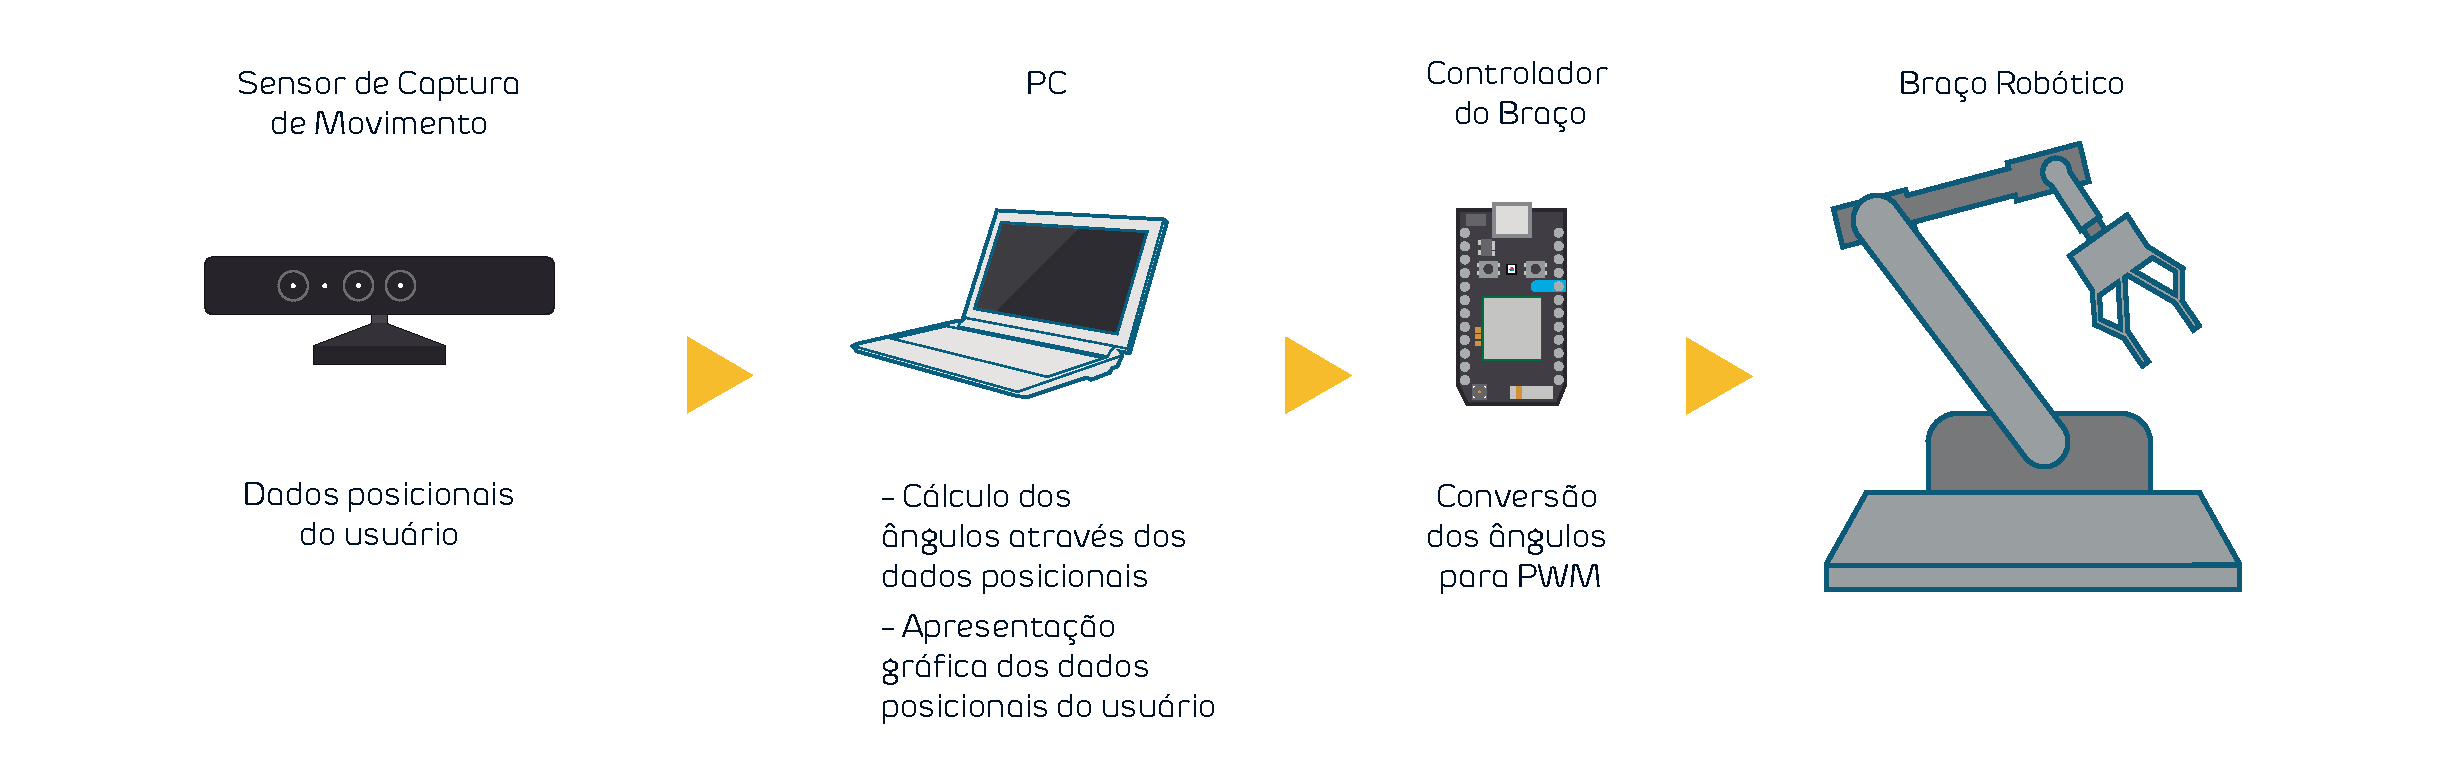
\includegraphics[width=\textwidth]{maniparm.pdf}	
		\end{center}
		\legend{Fonte: Autor}
	\end{figure}
	
	\subsubsection{Câmeras}\label{subsubsec-elementos-manip-cam}
	As imagens do ambiente remoto são capturadas por duas câmeras paralelas e enviadas a um servidor(\autoref{fig_manipcam}).
		\begin{figure}[h!]
		\caption{\label{fig_manipcam}  Manipulação de dados pelo sistema de câmeras estereoscópicas}
		\begin{center}
			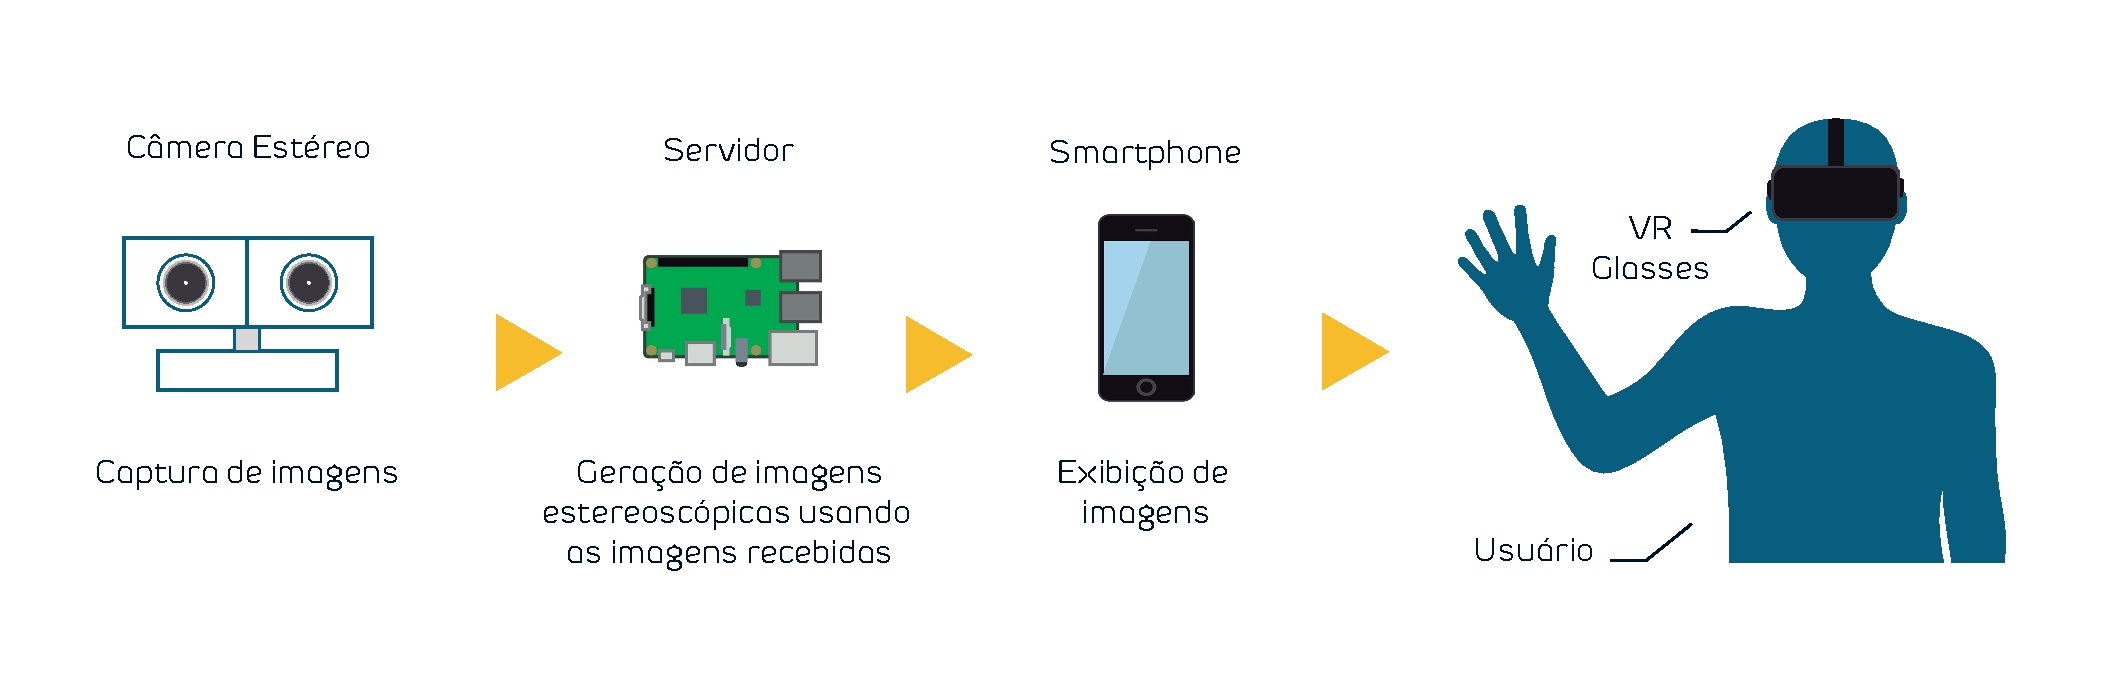
\includegraphics[width=\textwidth]{manipcam.pdf}	
		\end{center}
		\legend{Fonte: Autor}
	\end{figure}
	
	\subsubsection{Movimentação das Câmeras}\label{subsubsec-elementos-manip-cam-motors}
	Os dados de movimentação da cabeça do usuário são enviados para um Transmissor de ângulo de rotação(\autoref{fig_manipmotcam}).
			\begin{figure}[h!]
		\caption{\label{fig_manipmotcam}  Manipulação de dados pelo sistema de motores da câmera}
		\begin{center}
			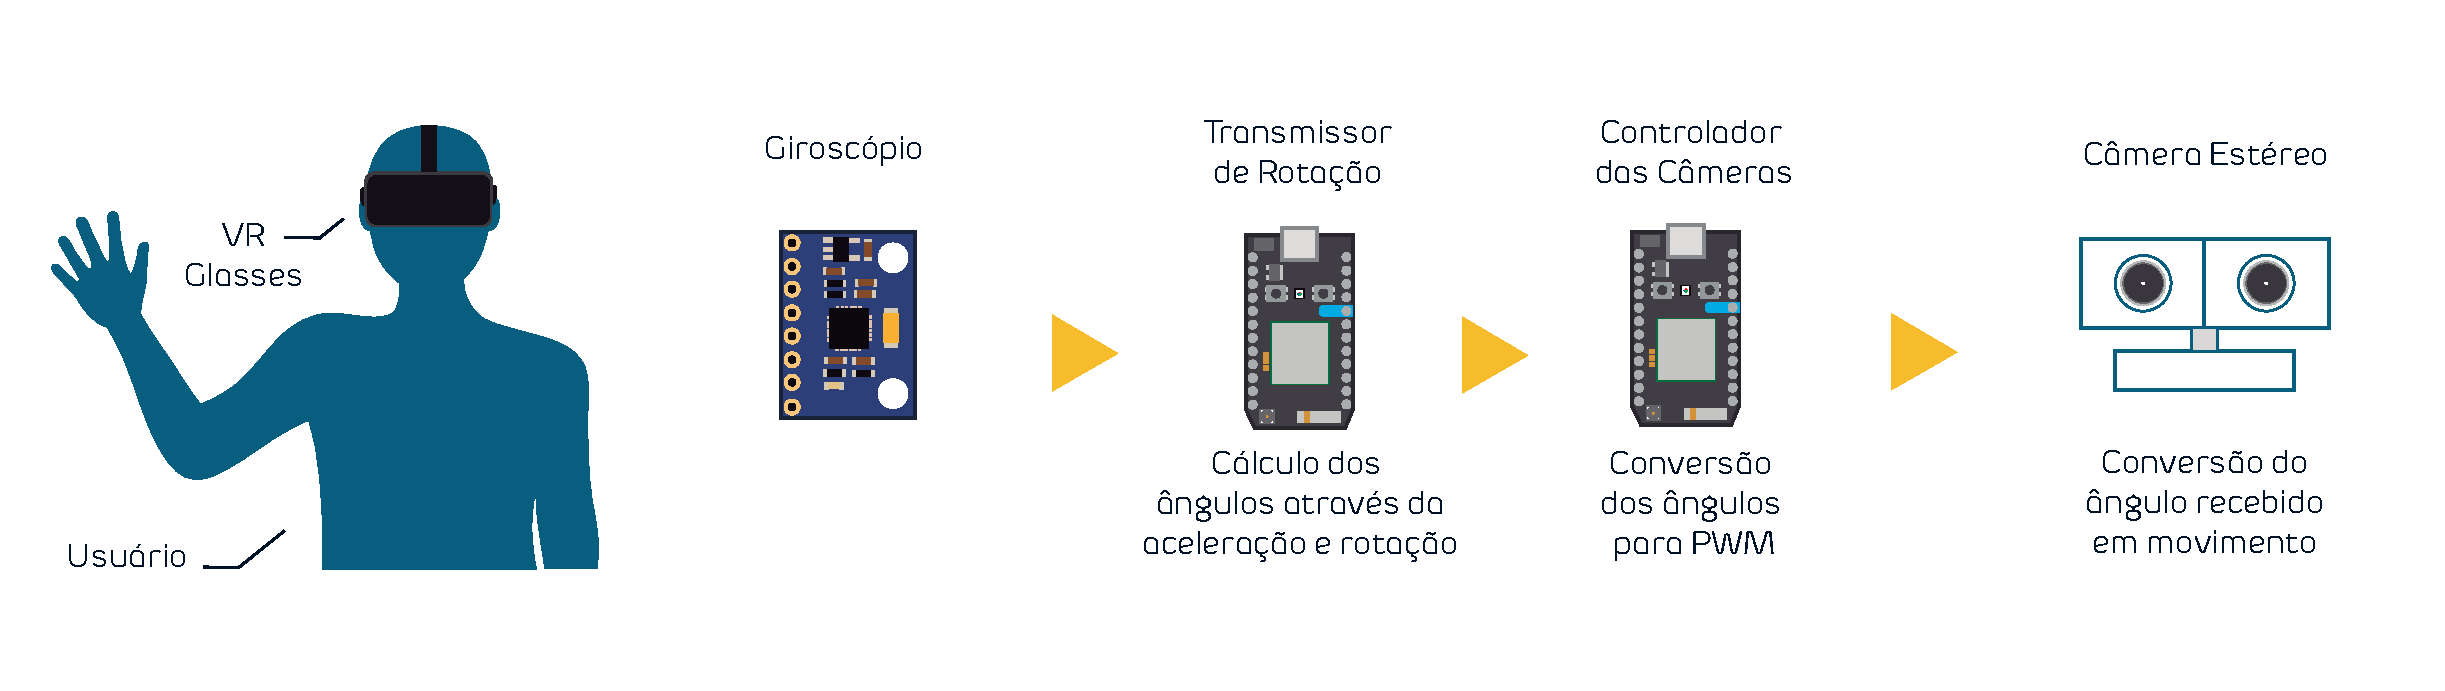
\includegraphics[width=\textwidth]{manipmotcam.pdf}	
		\end{center}
		\legend{Fonte: Autor}
	\end{figure}
	
	\subsection{Fluxo de informações}\label{subsec-fluxo-info}
	No projeto, todo o fluxo de informações entre os nós da arquitetura é unidirecional. Na \autoref{fig_techcom}, em cada flecha de comunicação, é mostrada de forma genérica a tecnologia utilizada entre os nós para troca de informações.
	As tecnologias para intercomunicação são as seguintes:
		\begin{figure}[h!]
		\caption{\label{fig_techcom}  Tecnologias Utilizadas para Conexão entre os Nós}
		\begin{center}
			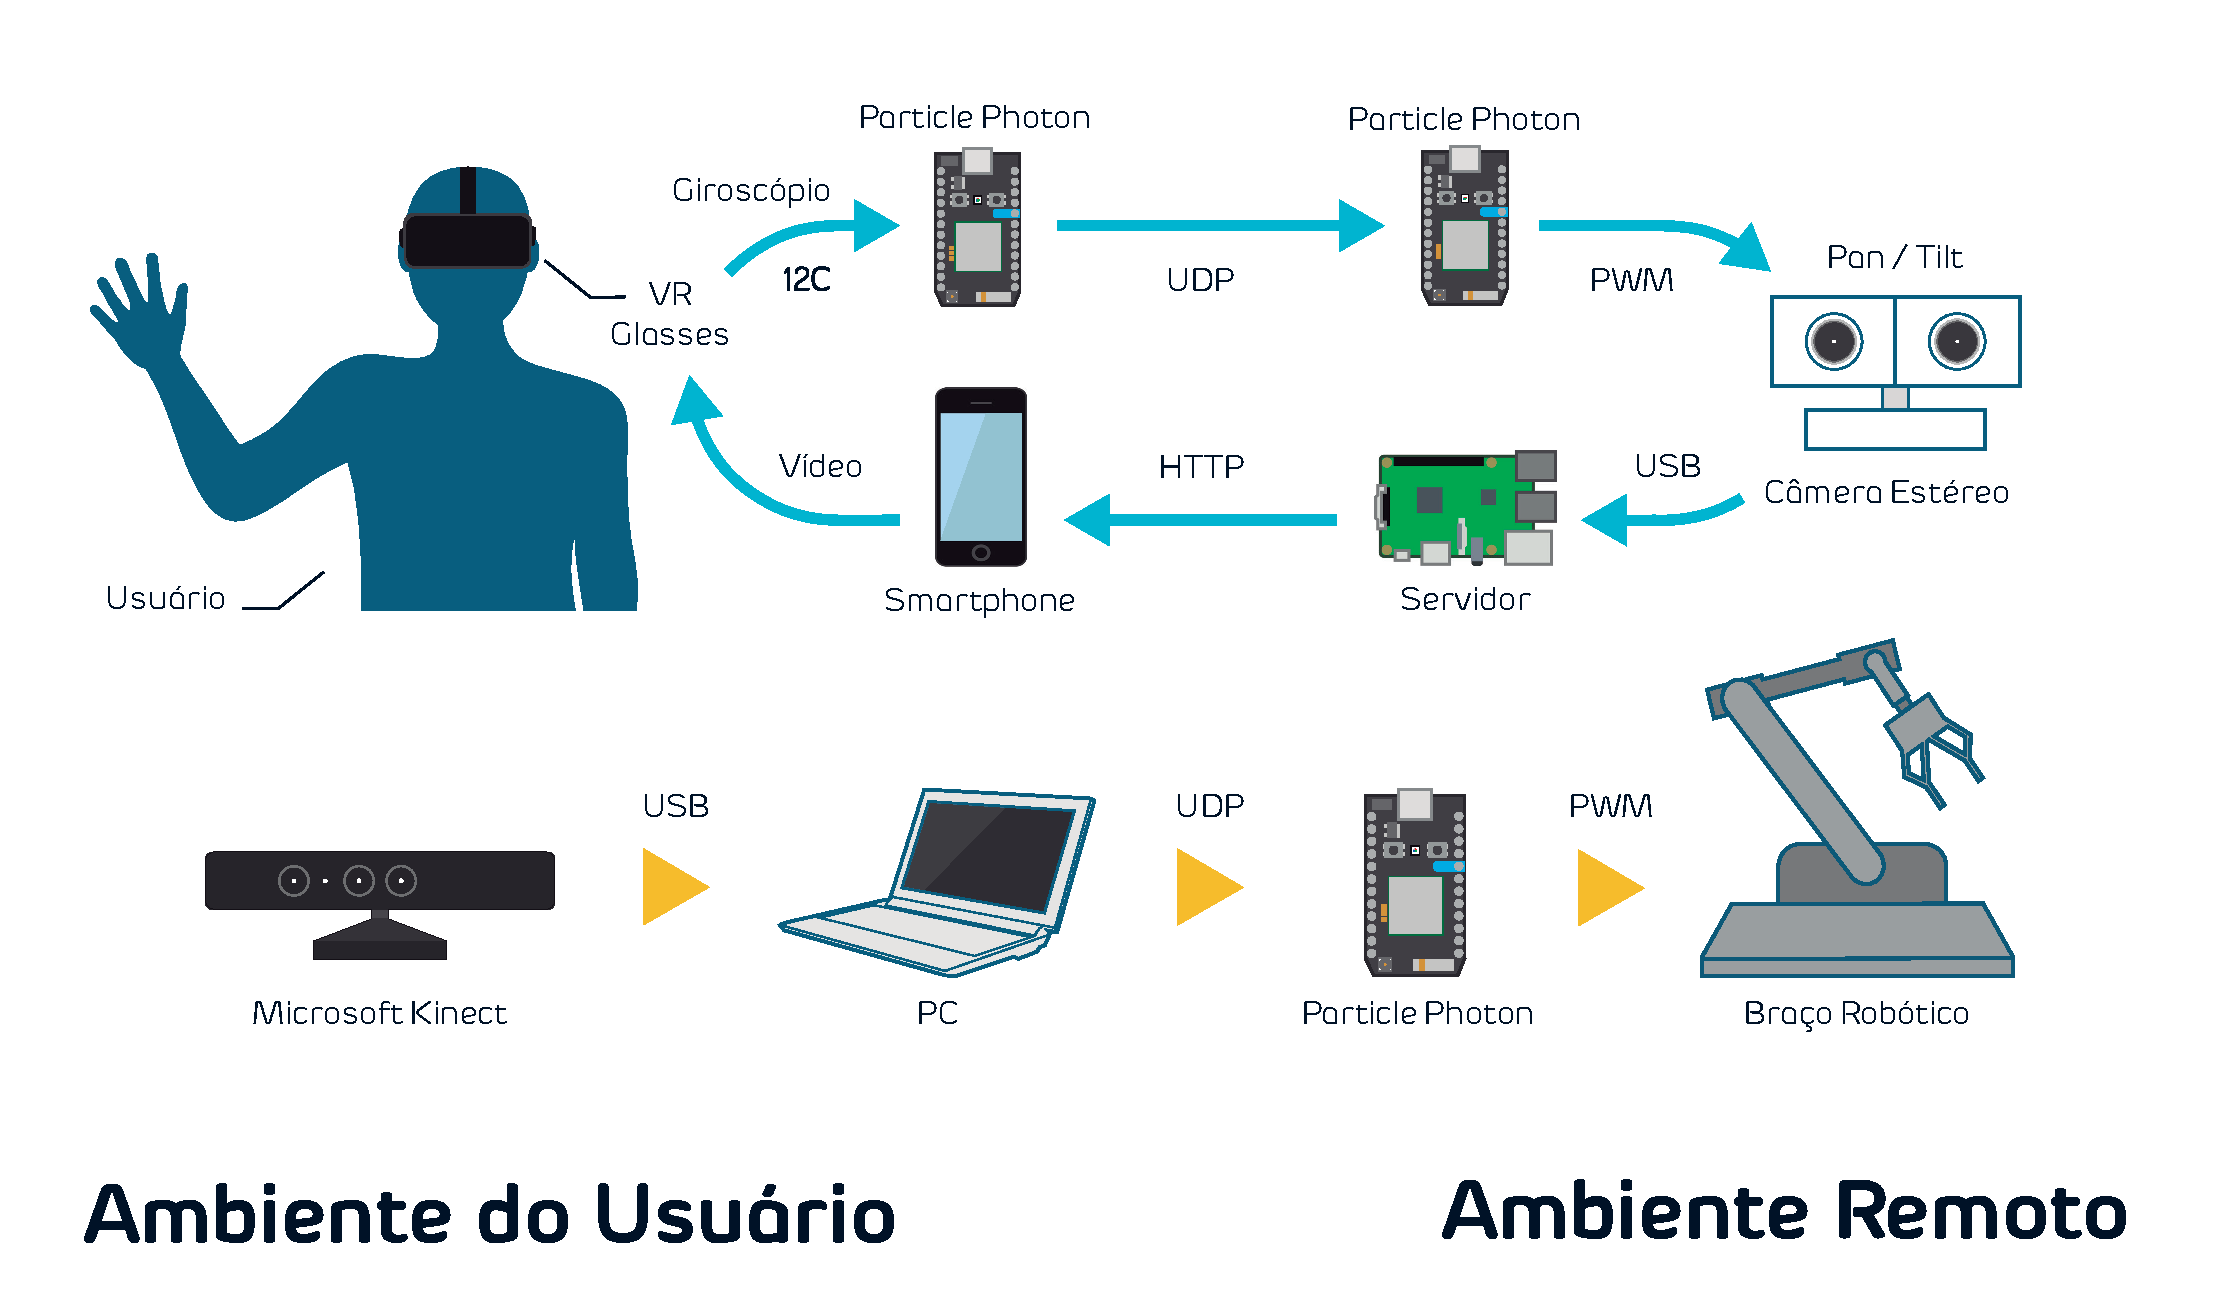
\includegraphics[width=\textwidth]{techcom.pdf}	
		\end{center}
		\legend{Fonte: Autor}
	\end{figure}
	
	\begin{itemize}[noitemsep]
		\item PWM - Link Cabeado: Comunicação entre os motores e o receptor de ângulos da câmera.
		\item PWM - Comunicação entre os motores e o receptor de ângulos do braço.
		\item Serial USB - Link Cabeado: Comunicação entre as câmeras e o servidor.
		\item Serial USB - Link Cabeado: Comunicação entre sensor de captura de movimento e o computador(servidor)
		\item Serial I2C - Link Cabeado: Comunicação entre giroscópio GY521 e Particle Photon. 
		\item HTTP TCP-IP- Link Internet: Uso do protocolo HTTP e TCP-IP para comunicação entre dispositivo móvel e servidor.
		\item Wireless UDP- Link Wireless: Uso do protocolo UDP  para comunicação entre transmissor de dados de rotação da cabeça do usuário e o controlador dos motores da câmera.
		\item Wireless UDP- Link Wireless: Uso do protocolo UDP  para comunicação entre o computador e o controlador do braço robótico.

	\end{itemize}

	As mensagens trocadas entre cada nó são detalhadas a seguir:
	
	\begin{itemize}
		\item Transmissor e Receptor da câmera: O transmissor de dados de rotação da cabeça do usuário envia ao o controlador dos motores da câmera mensagens com o seguinte formato:\par
		ângulos : { “rotação horizontal” : dados[0], “rotação vertical” : dados[1]}
\par
		\item  Giroscópio e Transmissor de ângulos de rotação: O giroscópio envia ao transmissor de dados de rotação da cabeça do usuário quaternion com o seguinte formato:
				ângulos : { “yaw” : dados[0], “pitch” : dados[1],“row” : dados[2], “rotation” : dados[3]}
		
		\item Transmissor e Receptor da câmera: O transmissor de dados de rotação da cabeça do usuário envia ao o controlador dos motores da câmera mensagens com o seguinte formato:\par
		ângulos : { “motor da base” : dados[0], “motor do ombro” : dados[1],“motor do cotovelo” : dados[2], “motor do pulso” : dados[3],“motor de rotação do pulso” : dados[4], “motor da garra” : dados[5]}
		
		\item  Receptor(ambos) e Motores: O receptor converte os dados recebidos em comandos PWM para os servo motores.
		
		\item  Câmeras e Servidor: As câmeras enviam imagens no formato JPEG para o computador em que o servidor se encontra(Raspberry Pi), que são coletadas pelo servidor.
		
		\item  Smartphone e Servidor: A aplicação utiliza o protocolo HTTP para realizar requisições ao servidor Apache pela internet.
		

		
\par

	\end{itemize}


	\section{Visão Computacional}\label{sec-comp}
	\subsection{Requisitos}\label{subsec-req}
	\subsubsection{Requisitos funcionais}\label{subsec-req-func}
	Nesta seção, apresentam-se os requisitos funcionais e não funcionais do sistema proposto.
\par
	\begin{center}
		\begin{tabular}{ | l |  p{7cm} |}
			\hline
			Identificação & RFB01  \\ \hline
			Nome & Captura de movimentos (braço)\\ \hline
			Descrição & O sistema deve suportar a captura da posição espacial das juntas do corpo do usuário
			\\ \hline
			Explicação & Os dados serão usados para o cálculo dos ângulos de movimentação do braço robótico  
			\\ \hline

		\end{tabular}
	\end{center}

	\begin{center}
	\begin{tabular}{ | l |  p{7cm} |}
		\hline
		Identificação & RFB02  \\ \hline
		Nome & Cálculo de ângulos (braço)\\ \hline
		Descrição & O sistema deve receber a posição espacial das juntas do corpo do usuário e através de trigonometria, calcular os ângulos de cada junta do braço do usuário
		\\ \hline
		Explicação & Os ângulos calculados serão transmitidos para o controlador dos motores do braço robótico  
		\\ \hline
		
	\end{tabular}
\end{center}
		\begin{center}
	\begin{tabular}{ | l |  p{7cm} |}
		\hline
		Identificação & RFB03  \\ \hline
		Nome & Visualização de ângulos\\ \hline
		Descrição & O sistema deve exibir o "esqueleto" do usuário e mostrar os ângulos em cada junta do braço
		\\ \hline
		Explicação & O sistema deve possuir uma interface gráfica que permita a verificação de captura dos dados e seu correto processamento em tempo real.
		\\ \hline
	\end{tabular}
\end{center}
	\begin{center}
	\begin{tabular}{ | l |  p{7cm} |}
		\hline
		Identificação & RFC01  \\ \hline
		Nome & Recepção de imagens(câmera)\\ \hline
		Descrição & O sistema deve receber as imagens das duas câmeras do sistema e disponibilizá-las ao servidor
		\\ \hline
		Explicação & As imagens serão juntadas pelo servidor em uma imagem estereoscópica, que será transmitida ao usuário
		\\ \hline
		
	\end{tabular}
\end{center}
		\begin{center}
		\begin{tabular}{ | l |  p{7cm} |}
			\hline
			Identificação & RFC01  \\ \hline
			Nome & Conversão de imagem\\ \hline
			Descrição & O sistema deve receber a imagem das câmeras e formatá-las de modo apropriado à visão estereoscópica
			\\ \hline
			Explicação & As duas imagens serão disponibilizadas lado a lado, de forma que sejam observadas como uma única imagem com profundidade quando o usuário vestir os óculos de realidade virtual.
			\\ \hline
		\end{tabular}
		\end{center}
				\begin{center}
				\begin{tabular}{ | l |  p{7cm} |}
					\hline
					Identificação & RFM01  \\ \hline
					Nome & Cálculo de ângulos(motores da câmera)\\ \hline
					Descrição & O sistema deve receber os dados de rotação e aceleração do giroscópio e calcular os ângulos em cada eixo com as devidas correções
					\\ \hline
					Explicação & Os ângulos calculados serão transmitidos para o controlador dos motores do braço robótico  
					\\ \hline
					
				\end{tabular}
			\end{center}


	\begin{center}
	\begin{tabular}{ | l |  p{7cm} |}
		\hline
		Identificação & RFM02  \\ \hline
		Nome & Cálculo de ângulos (motores da câmera)\\ \hline
		Descrição & O sistema deve receber a posição espacial das juntas do corpo do usuário e através de trigonometria, calcular os ângulos de cada junta do braço do usuário
		\\ \hline
		Explicação & Os ângulos calculados serão transmitidos para o controlador dos motores do braço robótico  
		\\ \hline
		
	\end{tabular}
\end{center}

	\subsubsection{Requisitos não funcionais}\label{subsec-req-nfunc}
		\begin{center}
	\begin{tabular}{ | l |  p{7cm} |}
		\hline
		Identificação & RNFB01  \\ \hline
		Nome & Taxa de envio de dados (braço)\\ \hline
		Descrição & O hardware de comunicação deve otimizar o número de requisições enviadas ao hardware de controle do braço.
		\\ \hline
		Explicação &  A taxa de envio de dados deve ser suficiente para que o o intervalo entre envios não seja perceptível, sem que sobrecarregue o hardware de controle.
		\\ \hline
		
	\end{tabular}
\end{center}	
		\begin{center}
	\begin{tabular}{ | l |  p{7cm} |}
		\hline
		Identificação & RNFB01  \\ \hline
		Nome & Taxa de envio de dados (Câmeras)\\ \hline
		Descrição & O hardware de captura de imagens deve otimizar o número de imagens enviadas ao servidor.
		\\ \hline
		Explicação &  A taxa de envio de dados deve ser suficiente para que o intervalo entre frames não seja perceptível, sem que sobrecarregue o servidor.
		\\ \hline
		
	\end{tabular}
\end{center}
	
		\begin{center}
		\begin{tabular}{ | l |  p{7cm} |}
			\hline
			Identificação & RNFM01  \\ \hline
			Nome & Taxa de envio de dados (motores da câmera)\\ \hline
			Descrição & O hardware de comunicação deve otimizar o número de requisições enviadas ao hardware de controle dos motores da câmera.
			\\ \hline
			Explicação &  A taxa de envio de dados deve ser  suficiente para que o intervalo entre envios não seja perceptível, sem que sobrecarregue o hardware de controle.
			\\ \hline
			
		\end{tabular}
	\end{center}

	\section{Visão da Engenharia/Infraestrutura}\label{sec-eng}
	Esta seção apresenta a arquitetura definida para a implementação do sistema.
	\subsection{Arquitetura do sistema}\label{subsec-arq}	
	\subsubsection{Sistema de Operação do Braço Mecânico}\label{subsec-arq-arm}

	\begin{figure}[h!]
		\caption{\label{fig_arq-arm}  Arquitetura do sistema de operação do braço robótico}
		\begin{center}
			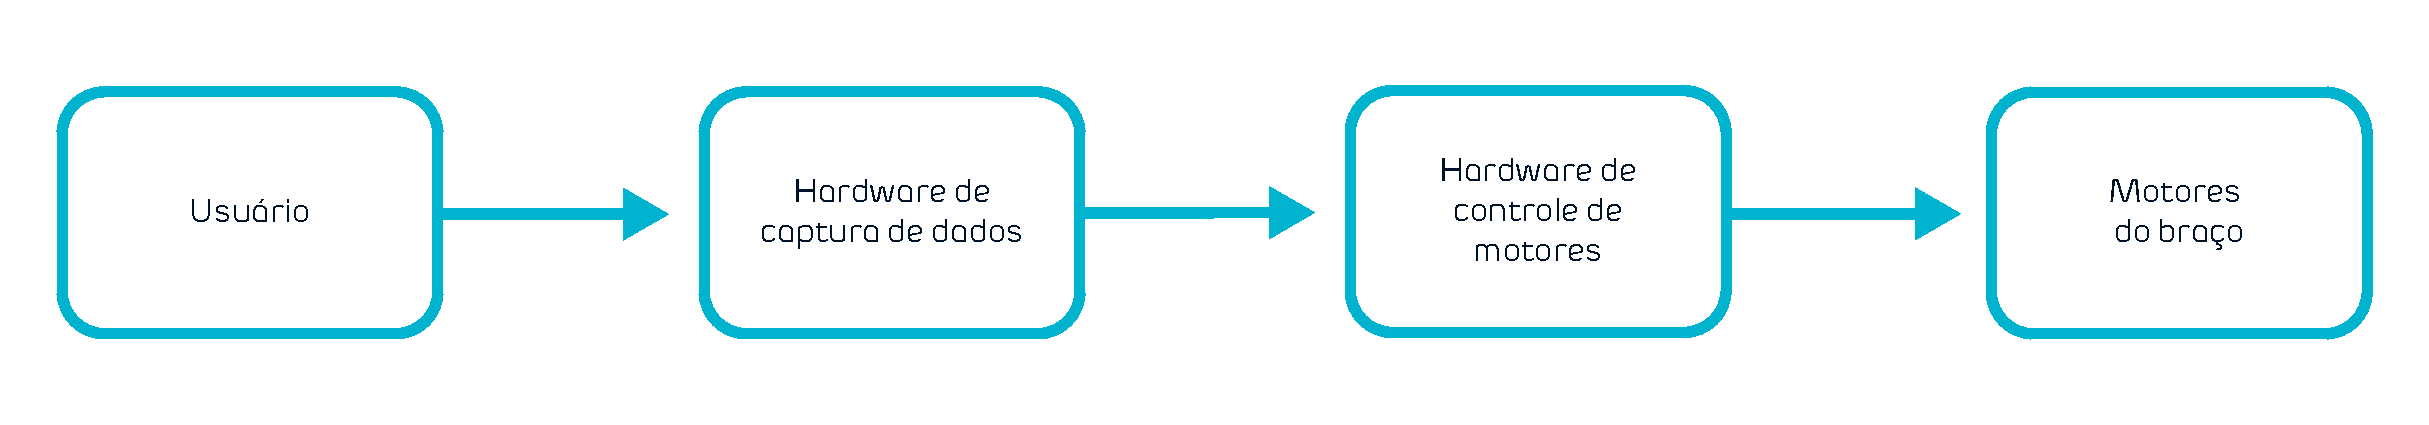
\includegraphics[width=\textwidth]{arq-arm.pdf}	
		\end{center}
		\legend{Fonte: Autor}
	\end{figure}
	
	\paragraph{Hardware de captura de dados}\label{par-arq-armcapture}
	É o hardware que realiza a interface com o usuário.
	Trata-se da parte responsável por coletar os dados relevantes de movimentação do braço do usuário, convertê-los para ângulos e enviá-los ao controlador do motor via protocolo UDP.\par

		\paragraph{Hardware de controle dos motores}\label{par-arq-armtranslate}
	É o hardware que realiza a interface com os motores, convertendo os dados recebidos em comandos PWM usados pelos motores.\par

	\subsubsection{Sistema de Operação do sistema de motores da câmera}\label{subsec-arq-mot}	

		\begin{figure}[h!]
		\caption{\label{fig_arq-mot}   Arquitetura do sistema de motores da câmera}
		\begin{center}
			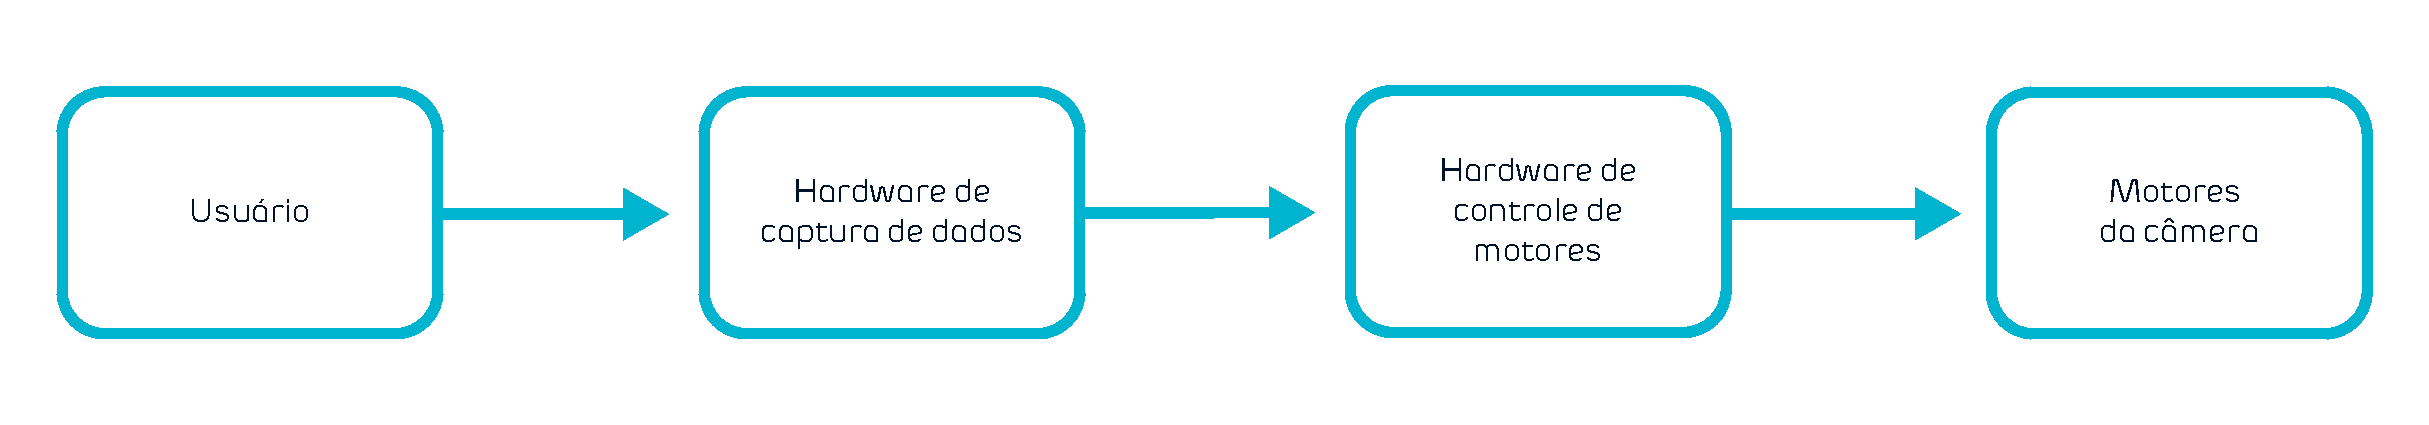
\includegraphics[width=\textwidth]{arq-mot.pdf}	
		\end{center}
		\legend{Fonte: Autor}
	\end{figure}
	\paragraph{Hardware de captura de dados}\label{par-arq-motcapture}
	Analogamente ao hardware do braço, é o hardware que realiza a interface com o usuário.\par
	Trata-se da parte responsável por coletar os dados relevantes de movimentação do braço do usuário, convertê-los para ângulos e enviá-los ao controlador do motor via protocolo UDP.\par
	\paragraph{Hardware de controle dos motores}\label{par-arq-mottranslate}
	Novamente, é o hardware que realiza a interface com os motores, convertendo os dados recebidos em comandos PWM usados pelos motores.\par

	\subsubsection{Sistema de Imagens Estereoscópicas}\label{subsec-arq-cam}
		\begin{figure}[h!]
		\caption{\label{fig_arq-cam}   Arquitetura do sistema de captura de imagens estereoscópicas}
		\begin{center}
			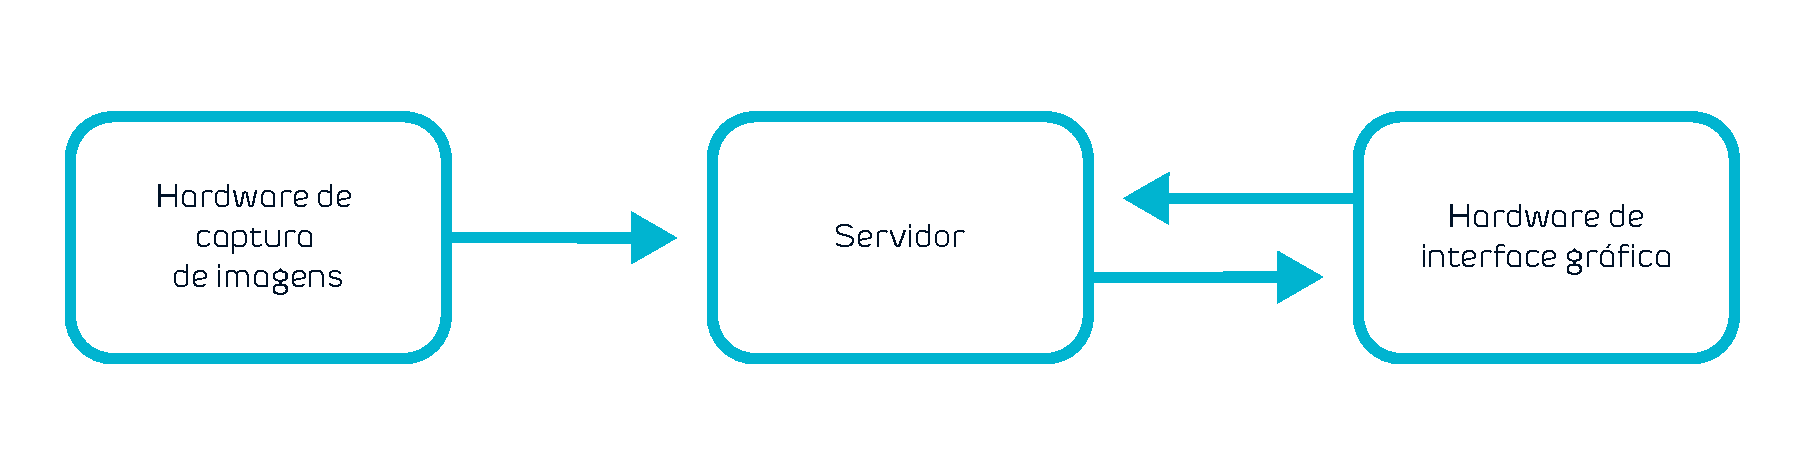
\includegraphics[width=\textwidth]{arq-cam.pdf}	
		\end{center}
		\legend{Fonte: Autor}
	\end{figure}
	\paragraph{Hardware de captura de imagens}\label{par-arq-cam}
	Realiza a captura de imagens do ambiente remoto e as disponibiliza para o servidor. 
	\paragraph{Servidor}\label{par-arq-server}
	Recebe as imagens e as reformata para que sejam vistas em um óculos de realidade virtual genérico como uma imagem estereoscópica.
	\paragraph{Hardware de interface gráfica}\label{par-arq-cell}
	Realiza a requisição de imagens ao servidor. Além disso, é responsável pela interface com o usuário, isto é, permite a visualização do ambiente remoto.

	\section{Visão Tecnológica}\label{sec-tec}
		\begin{figure}[h!]
		\caption{\label{fig_tech}  Visão tecnológica de Hardware do sistema}
		\begin{center}
			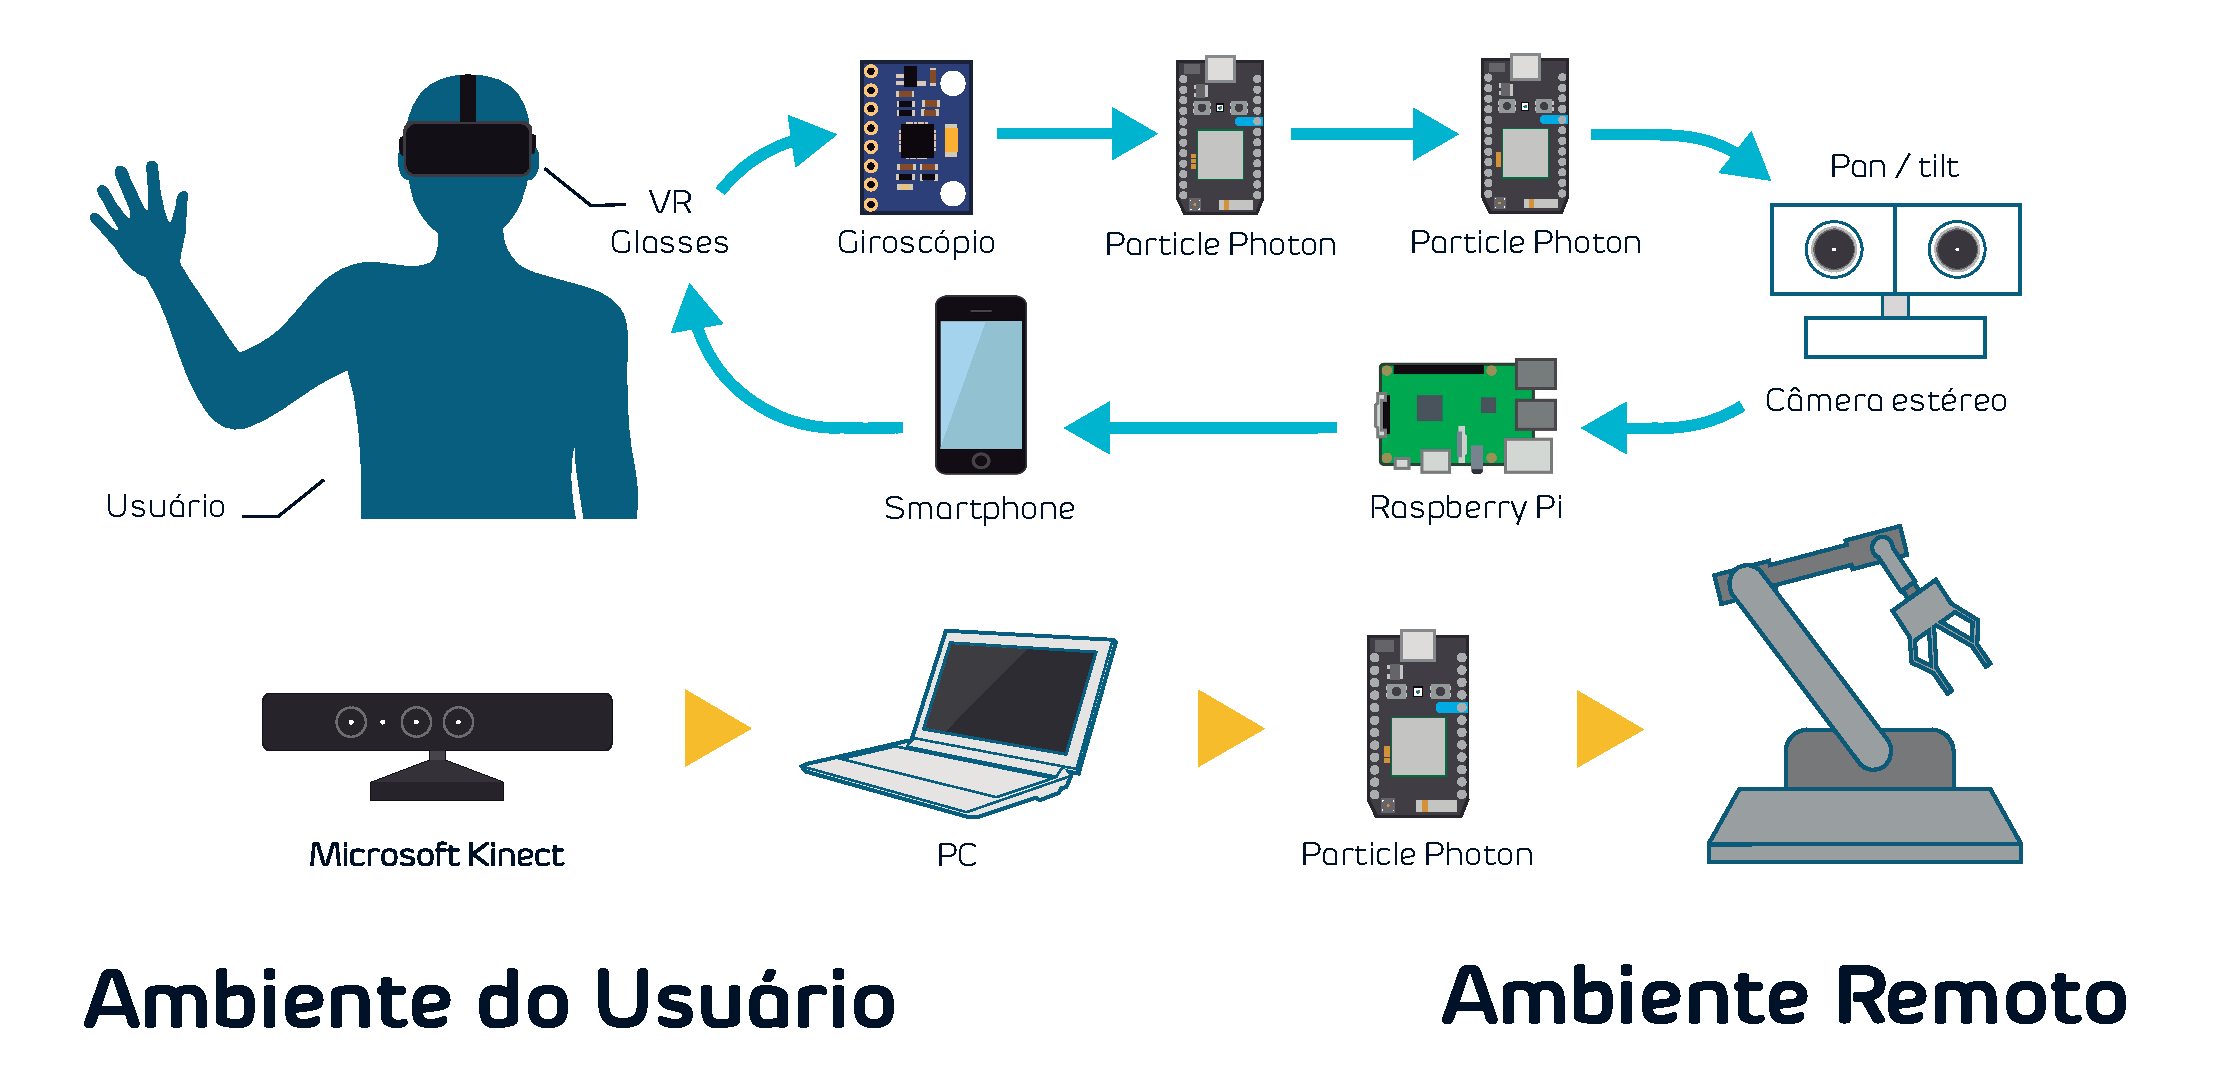
\includegraphics[width=100mm]{visaotecnologica.pdf}	
		\end{center}
		\legend{Fonte: Autor}
	\end{figure}
	Neste capítulo, são apresentadas as tecnologias utilizadas para cada camada do
	projeto, a partir da arquitetura definida no seção anterior . Posteriormente, são fornecidas informações básicas sobre cada tecnologia. As principais tecnologias utilizadas foram: Microsoft Kinect, Raspberry Pi, Particle Photon, GY521, Visual C\#, Apache HTTP Server, mjpg-streamer.\par
	

	\subsection{Microsoft Kinect}\label{subsec-kinect}
		 \begin{figure}[h!]
		\caption{\label{fig_kinectlogo}  Logotipo Kinect}
		\begin{center}
			\includegraphics[width=100mm]{kinect_logo.png}	
		\end{center}
		\legend{Fonte: Microsoft}
	\end{figure}
	 \begin{figure}[h!]
	\caption{\label{fig_kinect}  Kinect 2.0}
	\begin{center}
		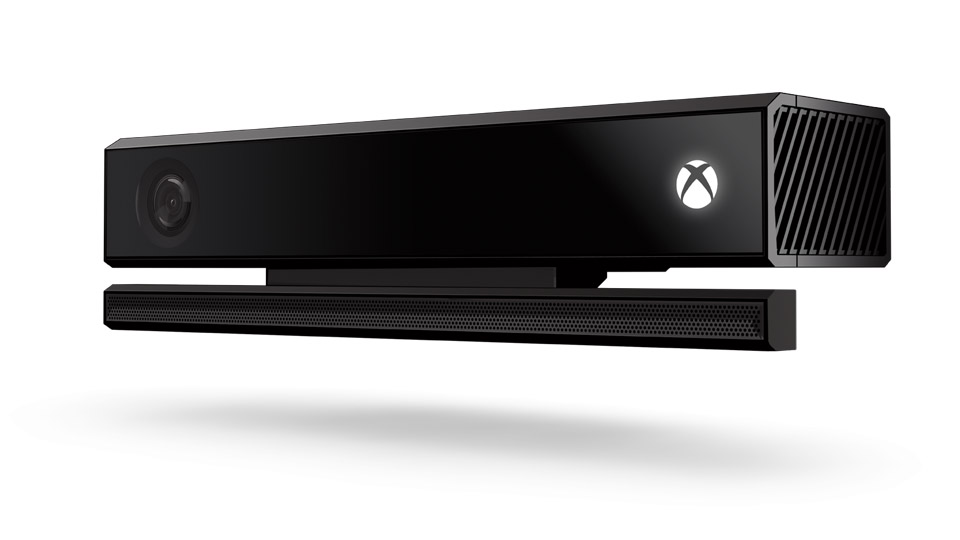
\includegraphics[width=100mm]{kinect20.jpg}	
	\end{center}
	\legend{Fonte: Microsoft}
\end{figure}
	Originalmente chamado Projeto Natal durante seu desenvolvimento, Kinect é uma linha de sensores de captura de movimento desenvolvida pela Microsoft em parceria com a Invensense para seus consoles Xbox 360 e Xbox one.\par

	Baseado em um periférico add-on estilo webcam, ele permite que os usuários controlem e interajam com seus consoles/computadores sem a necessidade de um controle remoto, através de uma interface natural do usuário usando gestos e comando por voz.
	A primeira geração do Kinect foi introduzida em novembro de 2010, com uma tentativa de expandir o público de Xbox 360 além do seu público gamer usual. 
	
	Uma versão para Windows foi lançada em 1 de fevereiro de 2012, e em 16 de junho de 2011 a Microsoft lançou o kit  de desenvolvimento de software do Kinect para Windows 7. Este SDK permitiu a desenvolvedores escreverem apps Kinect em C++/CLI, C\#, ou Visual Basic .NET.
	Atualmente, o Kinect encontra-se em sua segunda versão, com sua SDK na versão 2.0\cite{microsoft-kinect}.

	
	
	\subsection{Particle Photon}\label{subsec-photon}

		 \begin{figure}[h!]
		\caption{\label{fig_particle}  Logotipo Particle}
		\begin{center}
			
\includegraphics[width=100mm]{particle_logo.png}	
		\end{center}
		\legend{Fonte: Particle}
		\end{figure}
	 A Particle surgiu como uma campanha no Kickstarter em 2013 com a visão de desenvolvimento de Internet of Things simples e acessível e atualmente suas ferramentas são utilizados por 70 mil engenheiros em mais de 170 países e por várias companhias Fortune 500 para desenvolver e gerenciar diversos novos produtos IoT. Seu portfólio  de produtos inclui a Particle Cloud, uma infraestura de nuvem própria para os dispositivos da empresa, um cartão SIM e plano de datas próprios, os microcontroladores conectados via nuvem Electron e Photon e software exclusivo para desenvolvimento. A Particle foi listada em 2015 como uma das Fast Company’s Most Innovative Companies  e é listada em vários relatórios da Gartner em soluções IoT. \par
	\begin{figure}[h!]
	\caption{\label{fig_photon}  Particle Photon}
	\begin{center}
		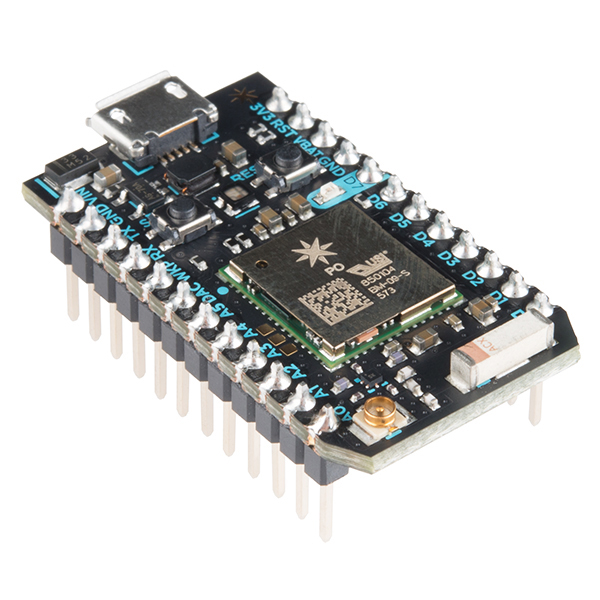
\includegraphics[width=70mm]{photon.jpg}	
	\end{center}
	\legend{Fonte: Particle}
\end{figure}		 	

	A Particle Photon, utilizada neste projeto é uma placa de prototipagem de hardware e software voltada a IoT baseada em um microcontrolador STM32 ARM Cortex M3 e um CI WiFi Broadcom BCM43362 totalmente desenvolvida pela Particle. A placa foi escolhida pela fácil programação, fator de forma e peso reduzidos e pela conectividade WiFi integrada\cite{Particle}. \par

		
	
	
	\subsection{GY521}\label{subsec-GY521}

	

	A placa GY521 é uma placa destinada a tornar a prototipação usando o CI MPU6050 mais fácil e prática ao integrá-lo em uma placa com saídas through hole.
	
	O CI MPU6050 é um dispositivo de rastreamento de movimento que contém um giroscópio de 3 eixos, um acelerômetro de 3 eixos e um Processador digital de movimento(DMP) em um encapsulamento de 4x4x0.9mm.
	 
	A MPU-6050 possui três conversores analógico-digitais de 16 bits (ADCs) para digitalizar as saídas do giroscópio e três 16-bit ADCs para digitalizar as saídas do acelerômetro. Para rastreamento de precisão de movimentos rápidos e lentos,  o giroscópio apresenta ranges programáveis pelo usuário de $\pm$250, $\pm$500, $\pm$1000, e $\pm$2000\degree/sec (dps) e o acelerômetro, ranges de $\pm$2g, $\pm$4g, $\pm$8g, e $\pm$16g. Um buffer on-chip FIFO de 1024 Bytes ajuda na redução de consumo de energia do sistema permitindo ao processador de sistema ler os dados do sensor em bursts e assim, entrar em um modo de baixa potência enquanto o MPU coleta mais dados.
	Comunicação com todos os registros de dispositivos são executadas utilizando ou I2C, ou 400kHz. Recursos adicionais incluem um sensor de temperatura acoplado e um oscilador on-chip com variação $\pm$ 1 \% na faixa de temperatura de operação. A peça possui uma robusta tolerância a choques de 10.000g e possui filtros passa-baixa programáveis para o giroscópio, o acelerômetro e o sensor de temperatura\cite{mpu6050}.
	

	
	\subsection{Raspberry Pi}\label{subsec-rasp}
	
		 \begin{figure}[h!]
		\caption{\label{fig_raspfound}  Logotipo Raspberry Pi}
		\begin{center}
			
\includegraphics[width=50mm]{raspberry-pi-logo.png}	
		\end{center}
		\legend{Fonte: Raspberry Pi Foundation}
	\end{figure}
	A ideia para um computador pequeno e barato para crianças surgiu em 2006, quando Eben Upton, Rob Mullins, Jack Lang e Alan Mycroft, do laboratório de computação da Universidade de Cambridge, ficaram preocupados com o declínio do nível dos estudantes do ensino médio que pleiteavam uma vaga para o curso de ciência da computação. Nos anos 90, os estudantes entrevistados para o curso tinham uma vasta experiência como programadores hobbystas, no entanto nos anos 2000 a situação mudou bastante os candidatos em sua maioria tinham algum conhecimento em web design.\par
	
			 \begin{figure}[h!]
		\caption{\label{fig_raspberry}  Raspbery Pi Modelo B versão 3}
		\begin{center}
			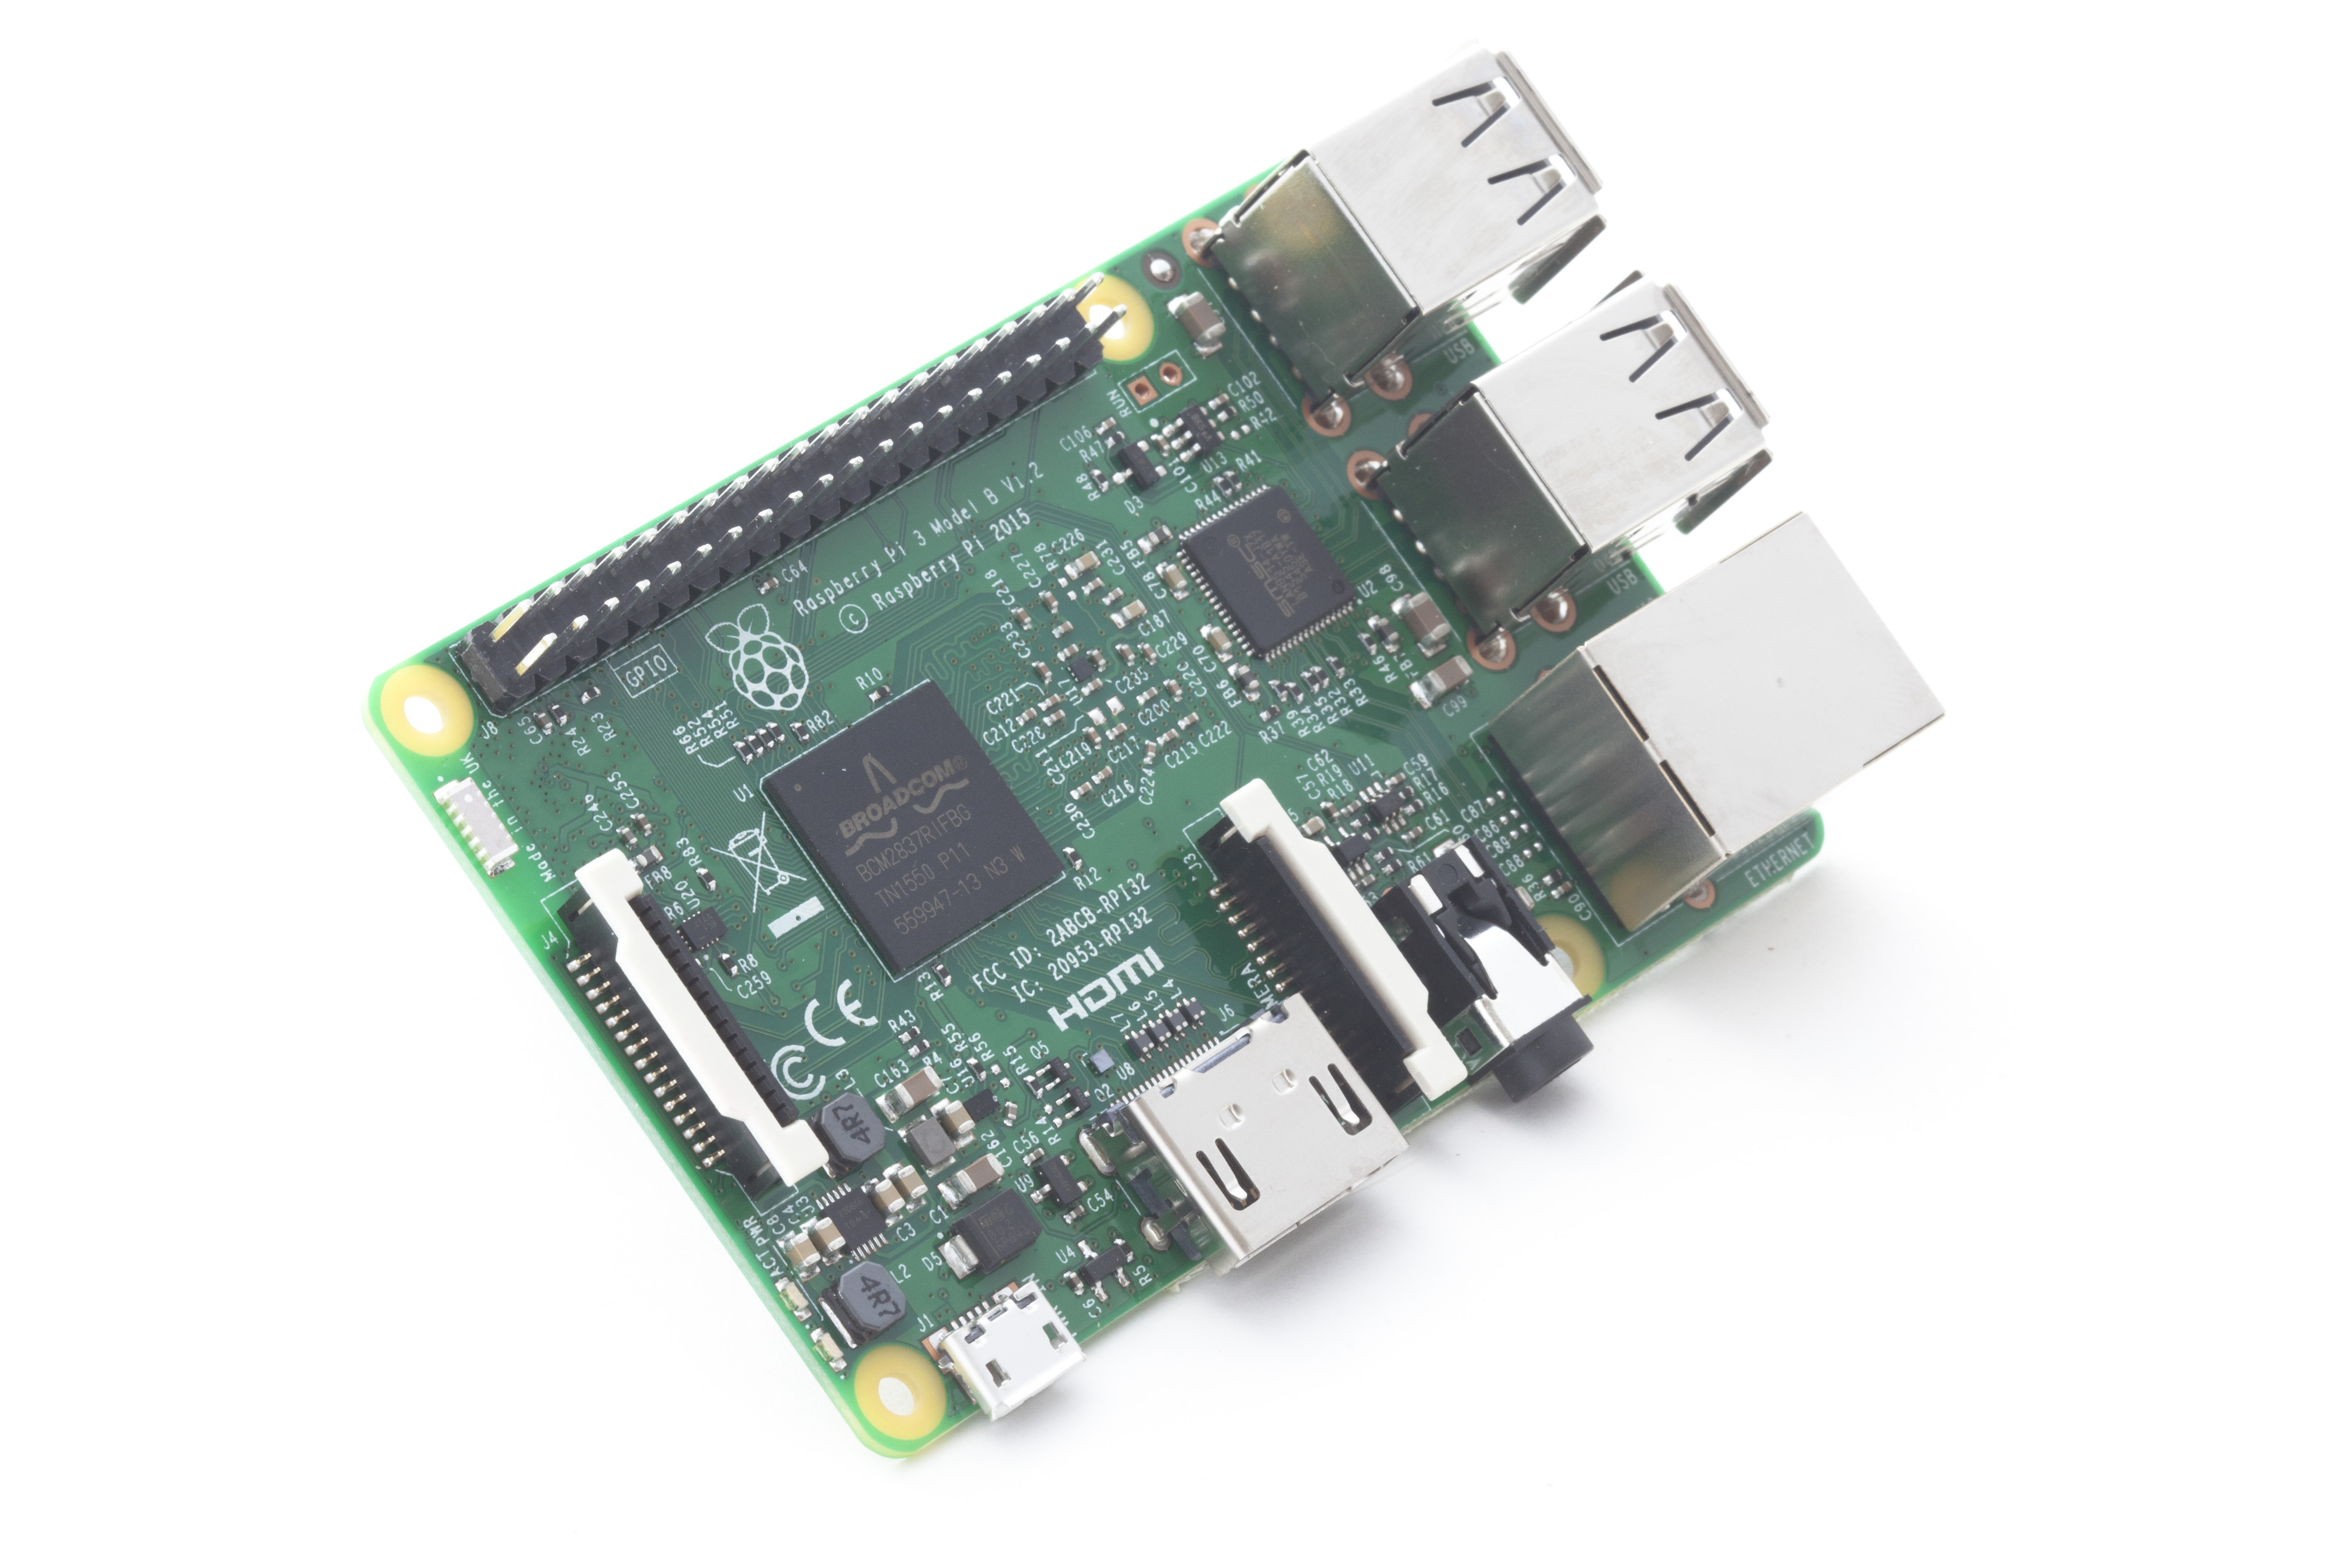
\includegraphics[width=100mm]{rasp3.jpg}	
		\end{center}
		\legend{Fonte: Raspberry Pi Foundation}
	\end{figure}
	
	O jeito como as crianças inglesas lidam com a tecnologia mudou. Alguns problemas foram encontrados: um grande número de aulas utilizando Word e Excel, ou escrevendo páginas web; o fim do crescimento da era ponto-com; e o crescimento dos PC’s e consoles de video-game, que substituíram as máquinas que as pessoas das gerações anteriores aprenderem a programar.\par
	Não há muito em que um pequeno grupo possa fazer para solucionar problemas como um currículo inadequado ou o fim de uma bolha financeira. Mas o grupo de Cambridge achou que podia fazer algo para mudar a situação em que os computadores se tornaram custosos e complexos e em que a programação neles teve que ser proibida pelos pais e assim pensaram em uma plataforma, que assim como os computadores pessoais antigos, podiam inicializar em um ambiente de programação. Então de 2006 a 2008, este grupo desenvolveu o que agora se tornou o Raspberry pi.\par
	Em 2008, os processadores desenvolvidos para telefones celulares se tornaram mais
	acessíveis, e com capacidade de processamento suficiente para prover multimídia, um
	recurso que poderia deixar a placa atraente para crianças, que não se interessariam por um dispositivo puramente voltado para programação.\par
	Foi então que foi criada a Fundação Raspberry pi, para transformar o projeto em
	realidade. Três anos depois o Raspberry pi modelo B entrou em produção em massa, e
	em dois anos vendeu mais de dois milhões de unidades.(...)\par
	
	O objetivo do Raspberry é difundir o uso de computadores de baixo custo, que
	possam ser utilizados para programação. Sendo uma tentativa de quebrar o paradigma que
	para ter acesso a internet é necessário comprar um computador de alto custo. Outra meta é a de que o uso dos computadores pessoais seja difundido entre as crianças. \cite{raspberry}.\par


	\subsection{Java}\label{subsec-java}
	
	O desenvolvimento em Processing é realizado utilizando-se Java, linguagem de programação orientada a objetos.
	Figura 31 – Logo da linguagem Java
		 \begin{figure}[h!]
	\caption{\label{fig_java}  Logo da linguagem Java}
	\begin{center}
		
\includegraphics[width=100mm]{java-logo-vector.png}	
	\end{center}
	\legend{Fonte: Oracle}
\end{figure}

	\subsubsection{História}\label{subsubsec-histjava}
	Java foi iniciado em junho de 2001, em um projeto liderado por James Gosling, Mike Sheridan e Patrick Naughton, sendo originalmente projetado para televisão interativa.\par
	Inicialmente, a linguagem era chamada Oak, referência ao carvalho (oak) plantado no exterior do escritório de Gosling. Mais tarde, a linguagem foi chamada de Green e, por fim, Java.\par
	A primeira implementação pública do Java (Java 1.0) foi lançada em 1995, pela Sun Microsystems. Nesta época, os principais navegadores incorporaram a execução de Java applets nas páginas web. Posteriormente, com o lançamento da versão Java 2, aumentou o número de plataformas e configurações compatíveis. A versão destinada à Desktops foi denominada JM2SE (Java Standard Edition), enquanto as aplicações de empresas eram desenvolvidas utilizando-se a tecnologia J2EE (Java Enterprise Edition). Por sua vez, a versão J2ME (Java Mobile Edition) oferecia recursos especificamente para aplicações de celulares. Posteriormente, por motivos de marketing, as versões foram renomeadas Java SE, Java EE e Java ME.\par
	Atualmente, o Java SE encontra-se na versão 8.0, e é considerada ainda como uma das mais utilizadas linguagens de programação.\cite{java}

	\subsubsection{Características da linguagem}\label{subsubsec-caractjava}
	O código Java é compilado em um bytecode, que é executado na máquina virtual java (JVM - Java Virtual Machine), independentemente da arquitetura da máquina.
	Possui gestão automática de memória, com uma implementação padrão de “Garbage Collector” que monitora as referências aos objetos em uma aplicação.
	Graças à grande popularidade da linguagem, existem inúmeras bibliotecas e frameworks disponíveis atualmente para o desenvolvimento de aplicações em Java. Dentre
	as funcionalidades oferecidas pelas bibliotecas mais utilizadas, destacam-se: IO (Input/Output), etworking (comunicação em rede), Concurrency (programação paralela),
	segurança, interfaces gráficas, etc.
	
	\subsection{Visual C\#}\label{subsec-csharp}
	 C\# é uma linguagem de programação de propósito geral orientada a objetos criada para o desenvolvimento de uma variedade de aplicações executadas sobre o .NET Framework.\par
	Seu time de desenvolvimento é conduzido por Anders Hejlsberg e sua versão mais recente é C\# 6.0, lançada em 2015.\par
	Já o Visual C\#, uma implementação da linguagem C\# pela Microsoft, é suportado por Visual Studio que possui um editor de código completo, compilador, modelos de projetos, designers, assistentes de código, um depurador poderoso e de fácil manuseio e entre outras ferramentas. \par
	A biblioteca de classes do .NET Framework fornece acesso a vários serviços do sistema operacional.\par
	\subsubsection{História}\label{subsubsec-histcsharp}
	

	Durante o desenvolvimento de .NET Framework, a biblioteca de classes foi originalmente escrita utilizando um sistema compilador de códigos gerenciados chamado Simple Managed C (SMC). Em janeiro de 1999, Anders Hejlsberg forma um time com o objetivo de construir uma nova linguagem que inicialmente foi nomeada Cool e posteriormente alterado para "C-like Object Oriented Language". Apesar de ter sido cogitado manter o nome "Cool" como nome final da linguagem , por questões de marca registrada esta ideia foi abandonada pela  Microsoft.\par
	Em 2000 quando o projeto .NET foi anunciado publicamente, a linguagem já havia sido renomeada para C\# e as bibliotecas de classes e a ASP.NET runtime  já haviam sido transferidoa para esta linguagem. O principal designer e arquiteto da C\# foi Anders Hejlsberg da Microsoft, que já havia participado no desenvolvimento de Turbo Pascal, Embarcadero Delphi (antigos CodeGear Delphi, Inprise Delphi e Borland Delphi), e Visual J++. \par\cite{visualc}
	\subsubsection{Características da linguagem}\label{subsubsec-caractcsharp}

	C\# foi projetado para se adequar a aplicações tanto em sistemas hospedados quanto embarcados, que vão desde grandes aplicações com sistemas operacionais sofisticadas até as menores com funções específicas. 
	Devido a estas características, tanto a linguagem como suas implementações devem fornecer suporte para princípios de engenharia de software como checagem strong type, checagem de array bounds, detecção de tentativas de utilização de variáveis não inicializadas e coletor de lixo automático. Robustez e durabilidade de software e a produtividade do programador são fatores importantes para a linguagem.

	Portabilidade é também uma característica muito importante para códigos-fonte e para programadores, especialmente para aqueles que já estão familiarizados com C and C++. 
		
	Finalmente, embora as aplicações C\# terem sidos planejadas para serem econômicas considerando a memória e requisitos de poder de processamento, a linguagem não se destina a competir diretamente em desempenho e tamanho com C ou Assembly.	
	  
	 
	\subsection{Protocolo HTTP}\label{subsec-http}
	
	HTTP (HyperText Transfer Protocol) é um protocolo da camada de aplicação para comunicação via internet. Trata-se de um protocolo do tipo requisição-resposta, baseado no modelo de computação cliente-servidor, no qual o cliente envia requisições ao servidor que, por sua vez, retorna uma reposta. Por exemplo, um navegador web é um cliente, enquanto um outro computador hospedando uma página web é o servidor.\par
	No contexto do modelo de camadas de redes, HTTP é um protocolo da camada de aplicação e é comumente utilizado em conjunto do TCP (Transmission Control Protocol), protocolo da camada de transporte.
	Dentre os métodos de requisições mais comuns, destacam-se:\par
	GET\par
	Requisita uma representação de um determinado recurso (uma página da internet, por exemplo). Requisições utilizando GET devem apenas recuperar dados e não ter outro efeito.\par
	POST\par
	Requisita que o servidor web aceite e salve os dados enviados no corpo (body) da mensagem enviada. É frequentemente utilizado ao fazer uploads de arquivos ou submeter formulários. Neste projeto, requisições do tipo GET são utilizadas para transmitir as imagens usando o servidor.\par

		\subsection{Servidor Apache HTTP}\label{subsec-apache}
		
					 \begin{figure}[h!]
			\caption{\label{fig_apachelogo}  Logo Apache HTTP Server}
			\begin{center}
				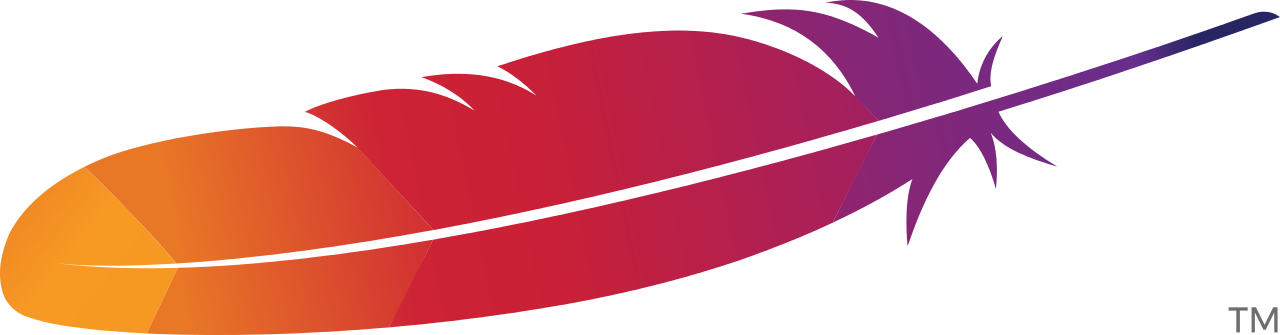
\includegraphics[width=100mm]{Apache_HTTP_server_logo_(2016).png}	
			\end{center}
			\legend{Fonte: Apache Software Foundation}
		\end{figure}
		O  Projeto Servidor Apache HTTP é um esforço de desenvolvimento de software colaborativo destinado a criar implementação de código fonte de servidor HTTP (Web) robusto, comercial, característico e disponível gratuitamente. O projeto é administrado em conjunto por um grupo de voluntários de diversos países, usando a internet e a web para comunicar, planejar e desenvolver o servidor e sua documentação relacionada.
		O Apache HTTP Server é um projeto da Apache Software Foundation.

	\subsubsection{Características}\label{subsubsec-caracteristicasapache}

	Lançado em 1995, o projeto Apache HTTP Server ("httpd") da fundação The Apache Software Foundation tem sido o servidor web mais popular desde abril de 1996, tendo sido celebrado o 20º aniversário do projeto em fevereiro de 2015.\cite{apache}
	
		\subsection{mjpg-streamer}\label{subsec-mjpg-streamer}	
		
		
		
	mjpg-streamer é uma aplicação de linhas de comando criada originalmente por Tom Stöveken para linux que copia frames JPEG de uma ou mais fontes para múltiplos output plugins. Pode ser usada para transmitir arquivos JPEG  através de uma webcam conectada a uma rede baseada em IP para vários tipos de software capazes de receber transmissões MJPG ao mesmo tempo.
	\subsubsection{Características}\label{subsubsec-histmjpg}
	Originalmente escrito para aparelhos embarcados com memórias RAM e CPU limitadas, uvc\_streamer(programa predecessor ao mjpg-streamer)  foi criado devido ao fato de câmeras compatíveis com Linux-UVC produzirem diretamente dados em JPEG, o que  permitia uma transmissão M-JPEG rápida e de com performance considerável.
	 Hoje, mjpg-streamer tem suporte a uma variedade de dispositivos de entrada diferentes.\cite{mjpg}
